\documentclass[conference]{IEEEtran}

% =====================
% Packages (Minimal & General)
% =====================
\usepackage[pdftex]{graphicx}
\graphicspath{{figures/}}
\DeclareGraphicsExtensions{.pdf,.png,.jpeg}

\usepackage{amsmath, amssymb}
\usepackage{array}
\usepackage{booktabs}
\usepackage{url}

% Center figures by default
\makeatletter
\g@addto@macro\@floatboxreset\centering
\makeatother

\hyphenation{op-tical net-works semi-conduc-tor}

% =====================
% Document
% =====================
\begin{document}

% -------- Title --------
\title{\LARGE \textbf{HARP: Human-Aware Routing Policies for Multi-Stage Decision Pipelines}}

% -------- Authors --------
\author{
    \authorblockN{Rohit Kulkarni, Lagnajeet Panigrahi}
    \authorblockA{University of California, Berkeley}
}

\maketitle

% =====================
% Abstract
% =====================
\begin{abstract}
A concise summary of the motivation, approach, and main findings of the work.
Avoid citations and equations. Typically 150--250 words.
\end{abstract}

\hfill\break
{\small
\textbf{\textit{Keywords---}}
keyword1, keyword2, keyword3, keyword4
}

\IEEEpeerreviewmaketitle

% =====================
% I. Introduction
% =====================
\section{Introduction}

High-stakes institutional decision like medical insurance claims, 
immigration applications, and credit approvals are increasingly supported
by machine learning systems. In general, these systems are not fully 
automated decision makers. Instead, automated models are embedded inside
structured human review pipelines, where cases can be autonomously resolved
or escalated to one or more human reviewers depending on factors including
uncertainty, risk, and institutional constraints \cite{kleinberg2017,cowgill2019}.

This problem is called \textit{selective prediction}, where a model is
allowed to abstain on inputs where it has low confidence and defer to an
expert human decision-maker \cite{elyaniv2010, geifman2017}. Previous works
have studied selective classification and abstention, describing 
tradeoffs between prediction risk and coverage. Works such as \cite{geifman2017,fisch2024}
have developed confidence-based deferral policies with strong theoretical 
guarantees. These approaches have been shown to be effective in applications where the
alternative to automated prediction is a single, homogenous human expert.

However, real-world decision pipelines rarely conform to single-stage abstraction. In practice,
human review is heirarchical, where casis can be routed to reviewers with differing levels
of expertise, authority, and cost. For example, in insurance claim resolution, an application
may be resolved automatically, reviewed by a junior examiner, escalated to a senior specialist,
or forwarded to an administrative judge. Modelling deferral as a binary decision process does
not always model this system well as it obscures important tradeoffs between accuracy and
human resource allocation.

Previous work on algorithmic triage and human-AI collaboration has studied how automated systems
can allocate cases between humans and models \cite{raghu2019,mozannar2021,wilder2020}. While these
approaches acknowledge heterogenous human expertise, they focus on two-stage settings, rarely
on heuristic or fixed routing rules, or do not explicitly connect to the selective prediction
framework. As a result, existing methods provide limited guidance for designing multi-stage
pipelines under explicit budget constraints.

In this work, we introduce Human-Aware Routing Policies (HARP), a framework for selecive
prediction in multi-stage human-AI decision pipelines. Rather than making deferral a binary
action, HARP formulates decision making as a routing problem over a heirarchy of human reviewers
with increasing costs, with the objective of minizing system loss while also respective
human resource consstraints. 

We study this framework in the context of structured application review pipelines motivated by 
insurance claim pipelines, including Medicare and Social Security Disability Insurance claim resolution, where decisions are sequential,
resource constrained, and subject to high institutional stakes. This setting shows the limitations
of single-stage selective prediction and motivats the need for routing-aware decision policies.

Our work makes the following contributions:
\begin{itemize}
 \item contrib1
 \item contrib 2
 \item contrib 3
\end{itemize}

% Example figure
\begin{figure}[t]
\includegraphics[width=0.9\columnwidth]{example-image}
\caption{Example figure caption.}
\label{fig:example}
\end{figure}

% =====================
% II. Problem Formulation
% =====================
\section{Problem Formulation}

\subsection{Single Stage Policies}

We specifically study human-AI collaborative decision making in structured application 
review pipelines, where an automated system can either issue a decision or defer the 
decision to a human reviewer at some cost.

Let 
\[
\begin{aligned}
(x, y) &\sim D \parbox[t]{0.6\linewidth}{, where $D$ is the real world distribution over applications and ground-truth decisions}\\
x &\in \mathcal{X} \parbox[t]{0.6\linewidth}{, where $x$ is an application}\\
y &\in \mathcal{Y} \parbox[t]{0.6\linewidth}{, where $y$ is the ground truth decision}
\end{aligned}
\]

We consider a predictive model $f: \mathcal{X} \rightarrow \mathcal{Y}$ and a 
deferral policy $r: \mathcal{X} \rightarrow \{0, 1\}$, where
\[
\begin{aligned}
r(x) &= 0 && \parbox[t]{0.6\linewidth}{when the policy chooses to predict autonomously} \\
r(x) &= 1 && \parbox[t]{0.6\linewidth}{when the policy defers to a human for a cost $c_{h} > 0$.}
\end{aligned}
\]

When $r(x) = 0$, the automated system incurs cost $\mathcal{L}_{1}$, which is given by
\[
\mathcal{L}_{1}(f) = \ell(f(x), y),
\]
where $\ell$ is by convention 0-1 loss or cross-entropy.

When $r(x) = 1$, the system defers to a human for a human cost $c_h > 0$,
assuming that the human produces the correct decision. Therefore, the total system loss can 
be modeled as the expectation of a function of $f$ and $r$:
\begin{align}
\mathcal{L}(f, r) 
    &= \mathbb{E}_{(x,y) \sim D} \Big[ 
        \ell(f(x),y) \cdot \mathbf{1}\{ r(x) = 0 \} \notag \\
    &\qquad + c_h \cdot \mathbf{1}\{ r(x) = 1 \} 
       \Big]
\end{align}

In this selective prediction model, when the policy $r(x) = 0$, $f$ predicts autonomously. 
Over time, as $r(x)$ continues to be 1, $c_h$ will increase. Therefore, we can define a coverage
function of $r$ as follows:
\begin{align}
\mathrm{cov}(r) = \mathbb{E}_{(x,y) \sim D}[\mathbf{1}\{r(x)=0\}],
\end{align}
which describes the fraction for which the policy $r$ chooses for $f$ not to abstain.

When $r(x) = 0$, $f(x)$ is evaluated and we can define the conditional risk as the loss $\ell$
between $f(x)$ and $y$ for a given $(x, y) \sim D$. More formally, this is:
\begin{align}
\mathrm{risk}(f, r) = \mathbb{E}_{(x,y) \sim D}[\ell(f(x), y) \mid r(x) = 0],
\end{align}
which shows the conditional risk when $f$ autonomously makes the decision.

Based on this coverage function and the conditional risk $\mathcal{L}$, we can define a 
coverage-constrained optimization problem as follows:
\begin{align}
\label{eq:minbinary}
\min_{f,r} \;& \mathbb{E} \big[ \ell(f(x),y) \mid r(x) = 0 \big], &&
\text{s.t. } \mathrm{cov}(r) \geq \kappa, 
\end{align}
where $\kappa$ is the constraint for the fraction where $r(x) = 0$.

Therefore, we can apply a confidence-based threshold defined on the confidence from the output of $f$, 
which is traditionally just the max of the output of the sigmoid or softmax function if $f$ is a 
neural network.
Thus, we let:
\begin{align}
p_\theta(y | x) && \parbox[t]{0.5\linewidth}{be the predictive distribution of $f$}\\
\mathrm{conf}(x) = \max_{y}p_\theta(y | x) && \parbox[t]{0.5\linewidth}{be defined as the 
                                                                        confidence of a given 
                                                                        application-decision pair.}
\end{align}

We can then threshold the policy $r$ on the confidence function for a hyperparameter 
$\tau$ as follows:
\begin{align}
r_\tau(x) =
\begin{cases} 
0 & \text{if } \mathrm{conf}(x) \geq \tau, \\
1 & \text{if } \mathrm{conf}(x) < \tau
\end{cases}
\end{align}

\subsection{Extension to Multi-Stage Policies}

The optimization problem in Eq.~\eqref{eq:minbinary} is applicable when we have a binary decision of
using policy $f$ or abstaining and deferring to an arbitrary human reviewer. However, when we have a 
heirarchical set of $k$ human reviewers $H = \{0,1, \dots ,k\}$, each with increasing costs $c_{h_k}$, we have
$c_{h_k}$ increasing when $k \geq 1$.

For the purposes of this paper, single-stage refers to $|H| = 1$, and multi-stage is when $|H| > 1$. 
We extend the single stage-policy to multi-stage. In this case, we make a trivial change to the 
minimization problem in Eq.~\eqref{eq:minbinary} and the initial routing policy $r$.
Let 
\begin{align}
r_{m}: \mathcal{X} \rightarrow \{0, 1, \dots, k\} && \parbox[t]{0.5\linewidth}{be the multistage routing policy,} \\
\ell_s(x) && \parbox[t]{0.5\linewidth}{be the loss of sending $x$ to stage $s$,} \\
B && \parbox[t]{0.5\linewidth}{be the total budget constraint for the human resources available.}
\end{align}

We assume $\ell_0(x) = \ell(f(x), y)$ corresponds to the automated model loss, and 
$\ell_s(x) = c_{h_s}$ for $s \geq 1$, assuming human reviewers produce correct decisions.

Therefore, the constrained optimization problem we must solve is as follows:
\begin{align}
\label{eq:minmulti}
\min_{r_m} \;& \mathbb{E} \big[ \ell_{r_m(x)}(x)], &&
\text{s.t. } \mathbb{E} \big[c_{h_{r_m(x)}}] \leq B. 
\end{align}

\subsection{Stochastic Routing Policies}

In practice, stochastic routing allows for calculating gradients in optimization, where 
the system learns a probabilistic policy over decision stages. Rather than deterministically 
assigning an application $x$ to a single stage, we define 
a routing distribution $\pi_\phi(s \mid x)$ over stages $s \in \{0,1,\dots,k\}$, 
parameterized by $\phi$. For each input, a stage is sampled according to this distribution, 
allowing the routing policy to express uncertainty and to smooth decisions near stage boundaries.

Under this formulation, the expected system loss is given by
\begin{align}
\mathbb{E}_{(x,y)\sim D}
\left[
\sum_{s=0}^k \pi_\phi(s \mid x)\,\ell_s(x)
\right],
\end{align}
with an associated expected human cost
\begin{align}
\mathbb{E}_{x\sim D}
\left[
\sum_{s=0}^k \pi_\phi(s \mid x)\,c_{h_s}
\right].
\end{align}

Therefore, at training time the system is optimized stochastically, but during inference it is
deterministic.

% =====================
% III. Background / Related Work
% =====================
\section{Background and Related Work}

We overview selective clasification and prediction policies, algorithmic triage, 
and organizational resource management models in current literature. 

\subsection{Selective Prediction and The Reject Option}

The basis for HARP is selective prediction, where a classifier has a reject option to abstain from making a 
prediction when a defined uncertainty score is high \cite{elyaniv2010}. These works generally deal with the 
statistical modelling of the trade-off bewtween risk, which is the error rate, and coverage, the fraction of samples
classified by the autonomous model. While previous literature has established confidence-based thresholds with 
statistical guarantees \cite{geifman2017}, they typically treat abstention as the end-state of the system. However,
in institutional pipelines abstaining is not always the end of the decision, with several heirarchies of human 
reviewers analyzing samples for different costs.

\subsection{Calibrated Selective Classification (CSC) as a Baseline}

One of the main challenges in the model routing domain is ensuring that the error probability of a routing model is
accurately captured by model confidence scores. Work by \cite{fisch2024,angelopoulos2022} in Calibrated Selective Classification (CSC)
has developed methods to provide statistical guarantees on risk by calibrating confidence scores within a separate,
non-routing model.

While existing works in CSC typically focus on the binary "predict" or "defer" case, we extend these statistical
guarantees to serve as a multi-stage baseline. Specifically, by calibrating a sequence of thresholds to partition 
a confidence space into $n$ distinct regions, where $n$ represents the number of reviewers in the institutional heirarchy,
we create a strong calibration-based benchmark to compare with HARP's learned routing policies.

\subsection{Learning to Defer (L2D)}

Learning to Defer, or L2D, is a deferral policy where the automated decision-making model and the deferral 
policy should be optimized together to account for when there exists a human partner \cite{madras2018}. L2D generally assumes
a single-stage system with a homogenous pool of experts \cite{mozannar2021} or just one expert. Our work extends L2D by recognizing
that human expertise can be structured heirarchically, especially when cases are escalated to increasingly
accurate human reviewer and higher costs are incurred on the institution.



% =====================
% IV. Data, Materials, or Methods
% =====================
\section{Data Processing}

To evaluate the HARP framework, we collect raw administrative
medical records from the Centers for Medicare and Medicaid 
Service Medicare Claims Synthetic Public Use Files (CMS DE1.0 SynPUF 2008-2010).
We develop a data pipeline to structure these raw claims in a multi-stage
decision environment.

\subsection{Assigning Reviewer Heirarchies}

In order to assign learnable reviewer heirarchies, we treat
a reviewer $n$ to have a higher complexity than the previous
reviewer $n-1$, where a complexity score $S(x)$, for each claim
$x$, is defined as:

\begin{align}
    S(x) = \sum_{i \in \text{indicators}} w_i \cdot 1_i(x),
\end{align}

where $w_i$ is the weight for the respective indicator and
for the indicator function $1_i(x)$ active when claim $x$ meets any indicator below:

\begin{itemize}
\item multi-payer involvement
\item a short-stay duration of less than one day
\item any completed surgical operation
\item a high-cost bill defined as $>$\$20,000
\end{itemize}

\begin{figure}[h!]
    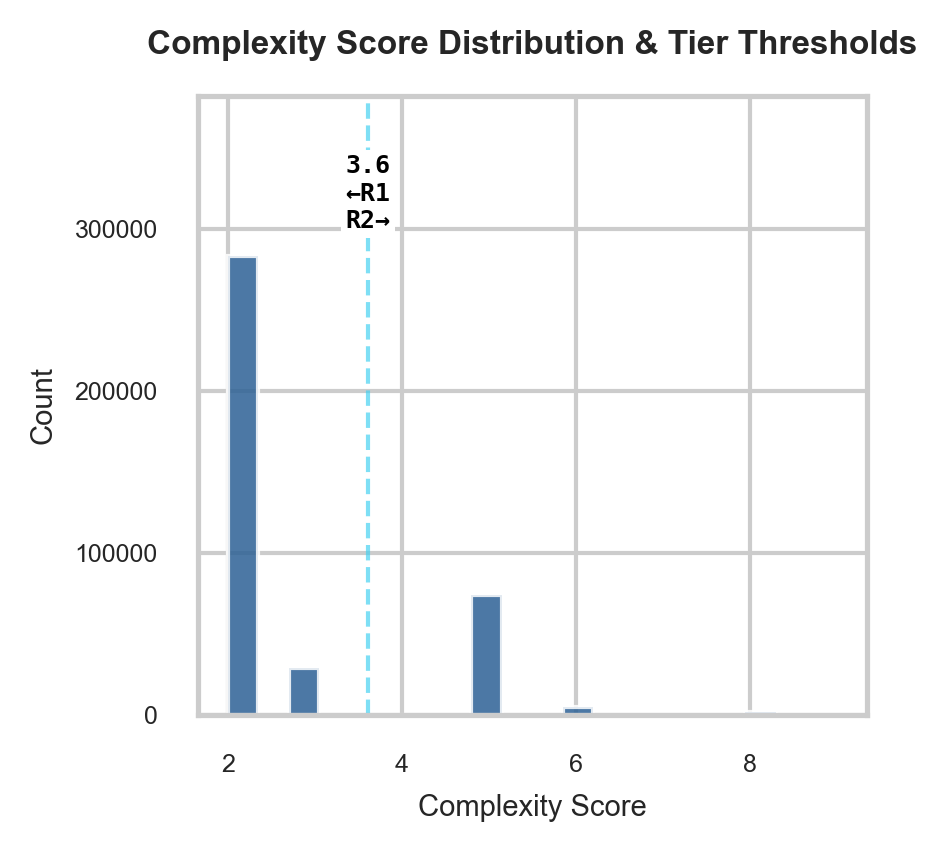
\includegraphics[width=0.9\columnwidth]{complexity_thresh.png}
    \caption{K-means determined thresholds between $n=2$ reviewer classes defined across the complexity scores}
    \label{fig:kmeansthresh}
\end{figure}

To partition the complexity scores for each claim into a heirarchy of $n$ reviewers, we apply K-means clustering
to the distribution of $S(X)$. Let $B = \{b_1, b_2, \dots, b_n\}$ be the set of K-means centroids, then we calculate
the threshold complexity scores between each reviewer tier $C = \{c_1, c_2, \dots, c_{n-1}\}$ as the midpoint
between the nodes in $B$, i.e.
\begin{align}
c_n = \frac{b_n + b_{n+1}}{2}.
\end{align}

\begin{figure*}[t]
    \centering
    \includegraphics[width=0.9\textwidth, height=0.3\textheight]{example-image-a}
    \caption{Human-Aware Routing Policies (HARP) model architecture. We use a shared encoder and frozen $f$ in order to train a router $\pi$ to learn the HARP routing policy.}
    \label{fig:harparchitecture}
\end{figure*}

\begin{figure}[h!]
    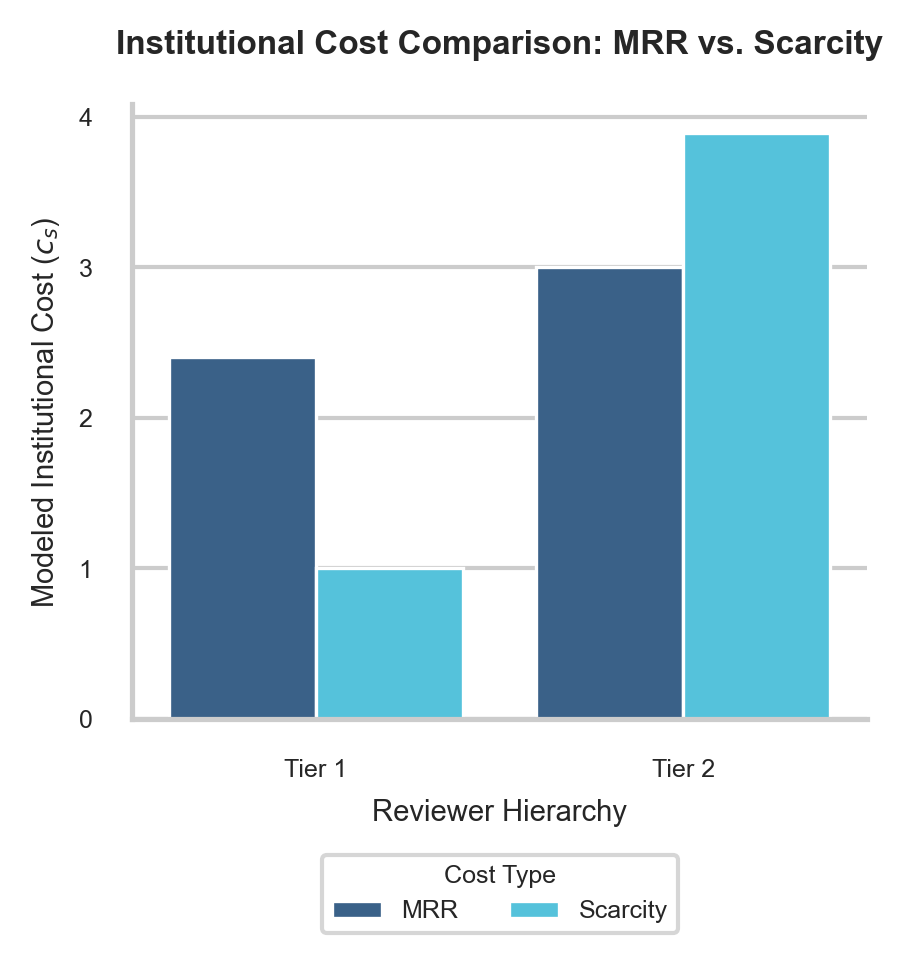
\includegraphics[width=0.9\columnwidth]{figures/mrr_v_scarcity.png}
    \caption{MRR costs vs. Scarcity costs across reviewer heirarchy show that MRR is best used in this dataset.}
    \label{fig:mrrbetter}
\end{figure}

\subsection{Determining Reviewer Performance and Costs \label{revcosts}}

With a real-world goverment dataset containing whether the $n$th reviewer escalates to the $n+1$th stage or makes a final decision,
we could statistically determine the costs of a specific reviewer. We model this by leveraging the claim complexity
score $S(X)$ and the reviewer's capabilities.

We predefine error rates $E = \{E_1, E_2, \dots, E_n\}$ for each reviewer tier, where reviewer $n = ||E||$ has a 5\%
error rate, since they must have the "final say" in the claim process and make a small percentage of administrative errors
that were not caught at stage $i < n$. 

We calculate costs for each reviewer stage up till $n$ reviewer stages as $c_s$ using two distinct methods:

\subsubsection{Marginal Risk Reduction (MRR)} is proportional to expected accuracy gain from escalating to a 
higher-tier reviewer. If $E_t$ is the error rate of reviewer tier $t < n$, then the cost of a reviewer at tier $t$ 
$c_t$ is defined as:

\begin{align}
    c_s = \lambda \cdot (E_{t-1} - E_{t}),
\end{align}

for a scaling factor $\lambda$.

\subsubsection{Scarcity} is inversely proportional to the frequency of a specific reviewer tier, so $c_t$ is defined
as:

\begin{align}
    c_t = c_{base} \cdot \frac{N_1}{N_t},
\end{align}

where $c_{base}$ is the base cost of reviewer 1. 

We use MRR for calculating $c_t$ due to since MRR can help HARP learn tangible accuracy gains in its cost, 
as shown by the increasing costs of MRR in fig. \ref{fig:mrrbetter}.


\section{Model Architecture}

As shown in fig. \ref{fig:harparchitecture}, HARP consists of three main models: a shared encoder, $f$, and $\pi$. $f$ is any automated model that outputs
accept/deny logits. First, $f$ and the encoder are trained as a warm-start. Once trained, $f$ and the encoder are frozen.
$\pi$ is the routing model HARP learns that takes the output of the frozen encoder and the entropy of $f$'s output
logit. Let $f$ output an accept logit for an encoded claim $x$, then the entropy of $f(x)$ is defined as the Binary Cross Entropy
of $f(x)$. 


\subsection{Routing and Loss Formulation}

As shown in fig. \ref{fig:harparchitecture}, HARP leverages the gumbel-softmax trick on $\pi(x)$ for a differentiable,
"discrete" routing choice. We use this to formulate a total system loss on which we optimize to train $\pi$.

We define the total system loss as
\begin{align}
    \mathcal{L}_{system} = r \cdot 1_g(0) + \sum_{i=1}^{n}  ((1_g(i) \cdot (1 - d_i)) \cdot \lambda_{\text{penalty}}) + c_i,
\end{align}

where $r$ is the binary cross entropy of $f(x)$, $1_g$ is an indicator function that is active if the 
gumbel softmax of $\pi(x)$ is 1 at index $i$, $d_i$ is if the reviewer at tier $i$ accurately identified the claim (0 or 1),
$\lambda_{\text{penalty}}$ is an error penalty hyperparameter, and $c_i$ is the institutional cost of a reviewer $i$
calculated by the methods described in sec. \ref{revcosts}.

We minimize this cost during training and during inference, we route by calculating $argmax(\pi(x))$ instead of
the gumbel-softmax.

% =====================
% V. Results
% =====================
\section{Results}

Present results objectively, using tables and figures where appropriate.

% =====================
% VI. Discussion
% =====================
\section{Discussion}

Interpret the results, explain trends, limitations, and unexpected outcomes.
Relate findings back to the motivation and prior work.

% =====================
% VI. Conclusion and Future Work
% =====================
\section{Conclusion and Future Work}

Summarize key contributions and outline potential directions for future research.

% =====================
% Author Notes
% =====================
\section*{Author Note}
The authors declare no competing interests.

% =====================
% References
% =====================
\bibliographystyle{IEEEtran}
\bibliography{refs}

\end{document}
